\section{Infrastruktur}
In Abbildung \vref{fig:Infrastruktur} ist die Infrastruktur der Webanwendung skizziert.

\begin{figure}[H]
	\centering 
	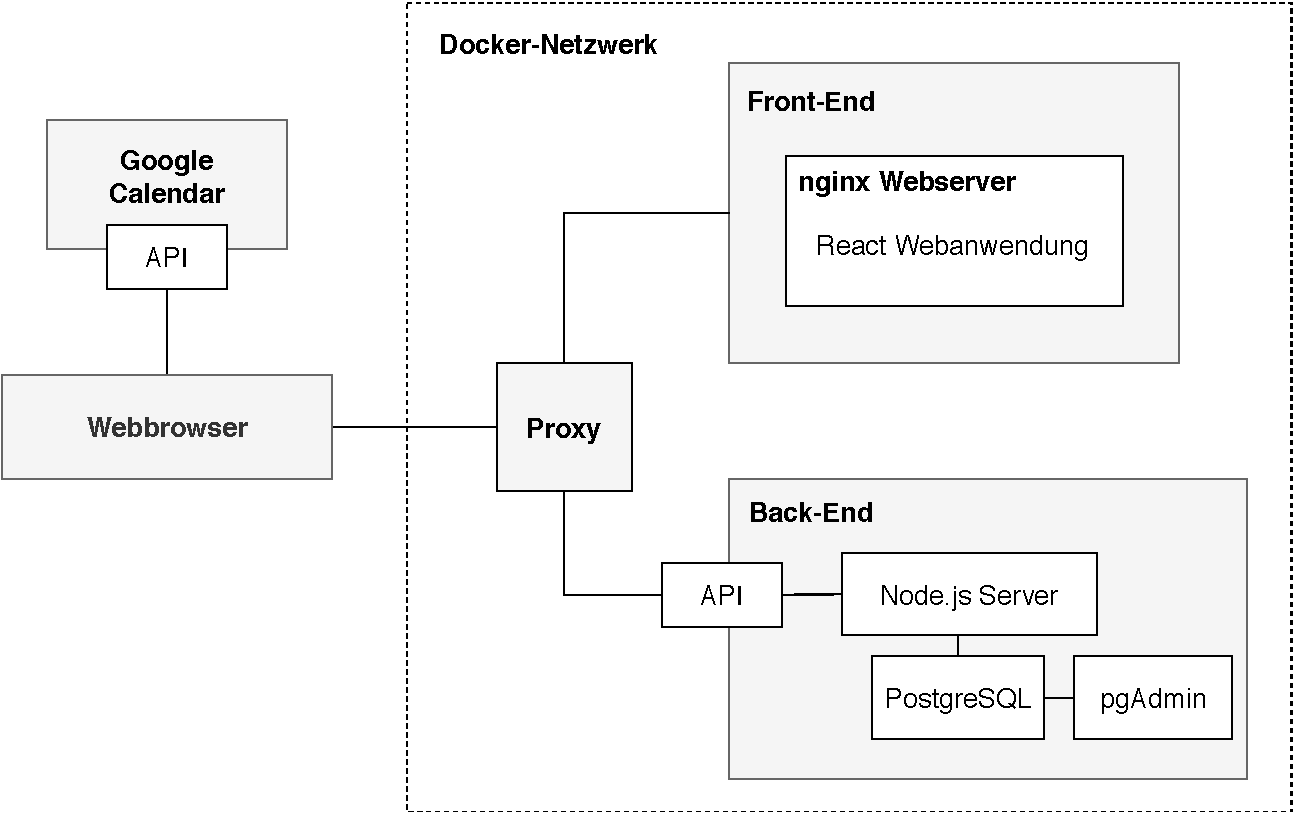
\includegraphics[width=\textwidth]{img/ImplementierungInfrastruktur.pdf}
	\caption[Übersicht der umgesetzen Infrastruktur]{\label{fig:Infrastruktur}Übersicht der umgesetzen Infrastruktur}
\end{figure}

\begin{itemize}
	\item Docker-Netzwerk bestehend aus mehreren Containern
		\subitem Docker-Compose alle hochgefahren etc.
		\subitem Container xyz für die Komponenten
		\subitem nochmal kurz: Wartbarkeit, Kapselung etc.
	\item Front-End: nignx Webserver für eine Webanwendung mit React 
	\item Back-End: 
		\subitem Node.js Server
		\subitem PostgreSQL in Verbindung mit PGAdmin 
		\subitem API-Schnittstelle nach außen, anfangs an REST orientieren; nicht konsequent aufgrund zeit
	\item Zentraler nginx Proxy: Kommunikation nach außen verschlüsselt; Kommunikation übernimmt NGINX-Proxy; Zertifikate für https- aktuell self-signed; Kommunikation im Docker-Netzwerk ist unverschlüsselt (HTTP)
	\item Webbrowser bleibt
	\item GC-API bleibt
\end{itemize}

\subsection{Github}
Für die Versionsverwaltung sowie das kollaborative Entwickeln wurden drei GitHub-Repositories erstellt. 
Front-End 
Back-End 
Dokumentation